%----------------------------------------------------------------------------------------
%	PACKAGES AND OTHER DOCUMENT CONFIGURATIONS
%----------------------------------------------------------------------------------------

%40pt,
\documentclass[a0, portrait]{a0poster}

\usepackage{multicol} % This is so we can have multiple columns of text side-by-side
\columnsep=100pt % This is the amount of white space between the columns in the poster
\columnseprule=3pt % This is the thickness of the black line between the columns in the poster

\usepackage[svgnames]{xcolor} % Specify colors by their 'svgnames', for a full list of all colors available see here: http://www.latextemplates.com/svgnames-colors

\usepackage{times} % Use the times font
%\usepackage{palatino} % Uncomment to use the Palatino font

\usepackage{graphicx} % Required for including images
\graphicspath{{figures/}} % Location of the graphics files
\usepackage{booktabs} % Top and bottom rules for table
\usepackage[font=small,labelfont=bf]{caption} % Required for specifying captions to tables and figures
\usepackage{amsfonts, amsmath, amsthm, amssymb} % For math fonts, symbols and environments
\usepackage{wrapfig} % Allows wrapping text around tables and figures

\definecolor{darkgreen}{RGB}{49,79,0}
%
%\usepackage{microtype}
%\DisableLigatures{encoding = *, family = *}

\begin{document}

%----------------------------------------------------------------------------------------
%	POSTER HEADER 
%----------------------------------------------------------------------------------------

% The header is divided into two boxes:
% The first is 75% wide and houses the title, subtitle, names, university/organization and contact information
% The second is 25% wide and houses a logo for your university/organization or a photo of you
% The widths of these boxes can be easily edited to accommodate your content as you see fit

\begin{minipage}[b]{0.8\linewidth}
\Huge \color{darkgreen} \textbf{An algorithm to recommend activities in scientific workflows:} \color{Black}\\ % Title
\huge\textit{An ontology, artificial inteligence and frequency-based approach}\\[2.5cm] % Subtitle
\Large \textbf{PhD Candidate Adilson Lopes Khouri \& \\  Associate Professor Luciano Antonio Digiampietri}\\[0.5cm] % Author(s)
\large \texttt{adilson.khouri.usp@gmail.com} \\
\large \texttt{digiampietri@usp.br}
\end{minipage}
\begin{minipage}[b]{0.20\linewidth}

\includegraphics[width=15cm]{USP.eps}\\
\end{minipage}

\vspace{0.5cm} % A bit of extra whitespace between the header and poster content

%----------------------------------------------------------------------------------------

\begin{multicols}{2} % This is how many columns your poster will be broken into, a portrait poster is generally split into 2 columns

%----------------------------------------------------------------------------------------
%	INTRODUCTION
%----------------------------------------------------------------------------------------

\section*{Introduction}

The number of research projects using intensive computing has been growing in areas in which scientists lack advanced computer skills such as biology, physics, and astronomy. One of the tools to assist in the management and construction of intensive computing experiments is the workflow management system. \emph{Scientific Workflows} represent structured and ordered processes, constructed manually, semi-automatically or automatically to solve scientific problems using activities, which can be: i) source code blocks; (ii) services; or iii) finished workflows. These systems facilitate the creation of new experiments, sharing of results and reuse of existing activities.

Nowadays, there are a large number of activities available in repositories such as \emph{myExperiment} which stores more than $2500$ workflows and \emph{BioCatalogue} which provides more than $2464$ services. The large number of activities and the low reuse of some activities and workflows motivate the construction of techniques to recommend activities to the scientists during the composition of workflows.

In the workflow management systems, activities are typically represented as graphical icons with drag and drop functionality. Thus, it is possible to construct computational experiments by dragging icons and filling in input parameters. Most of these systems provide sets of basic activities that can be used in different domains, for example, an activity that calculates the average value of a dataset is applicable in biology, physics, astronomy, and other areas. However, there is a precondition for reusing and\/or creating workflows: knowing the available activities.

In order to minimize the problem of knowing a large number of activities, several techniques were proposed to recommend activities or to compose workflows. In the first case, which aims to serve an expert user in these systems, during the construction of the workflow, activities are recommended to help to complete the workflow. In the second case, whose goal is to serve a less expert user on these systems, several workflows are built and the user should select which one most satisfies him\/her needs.
\begin{center}
\vspace{0.25cm} 
\large  \color{darkgreen} Related literature \\
\vspace{0.25cm}
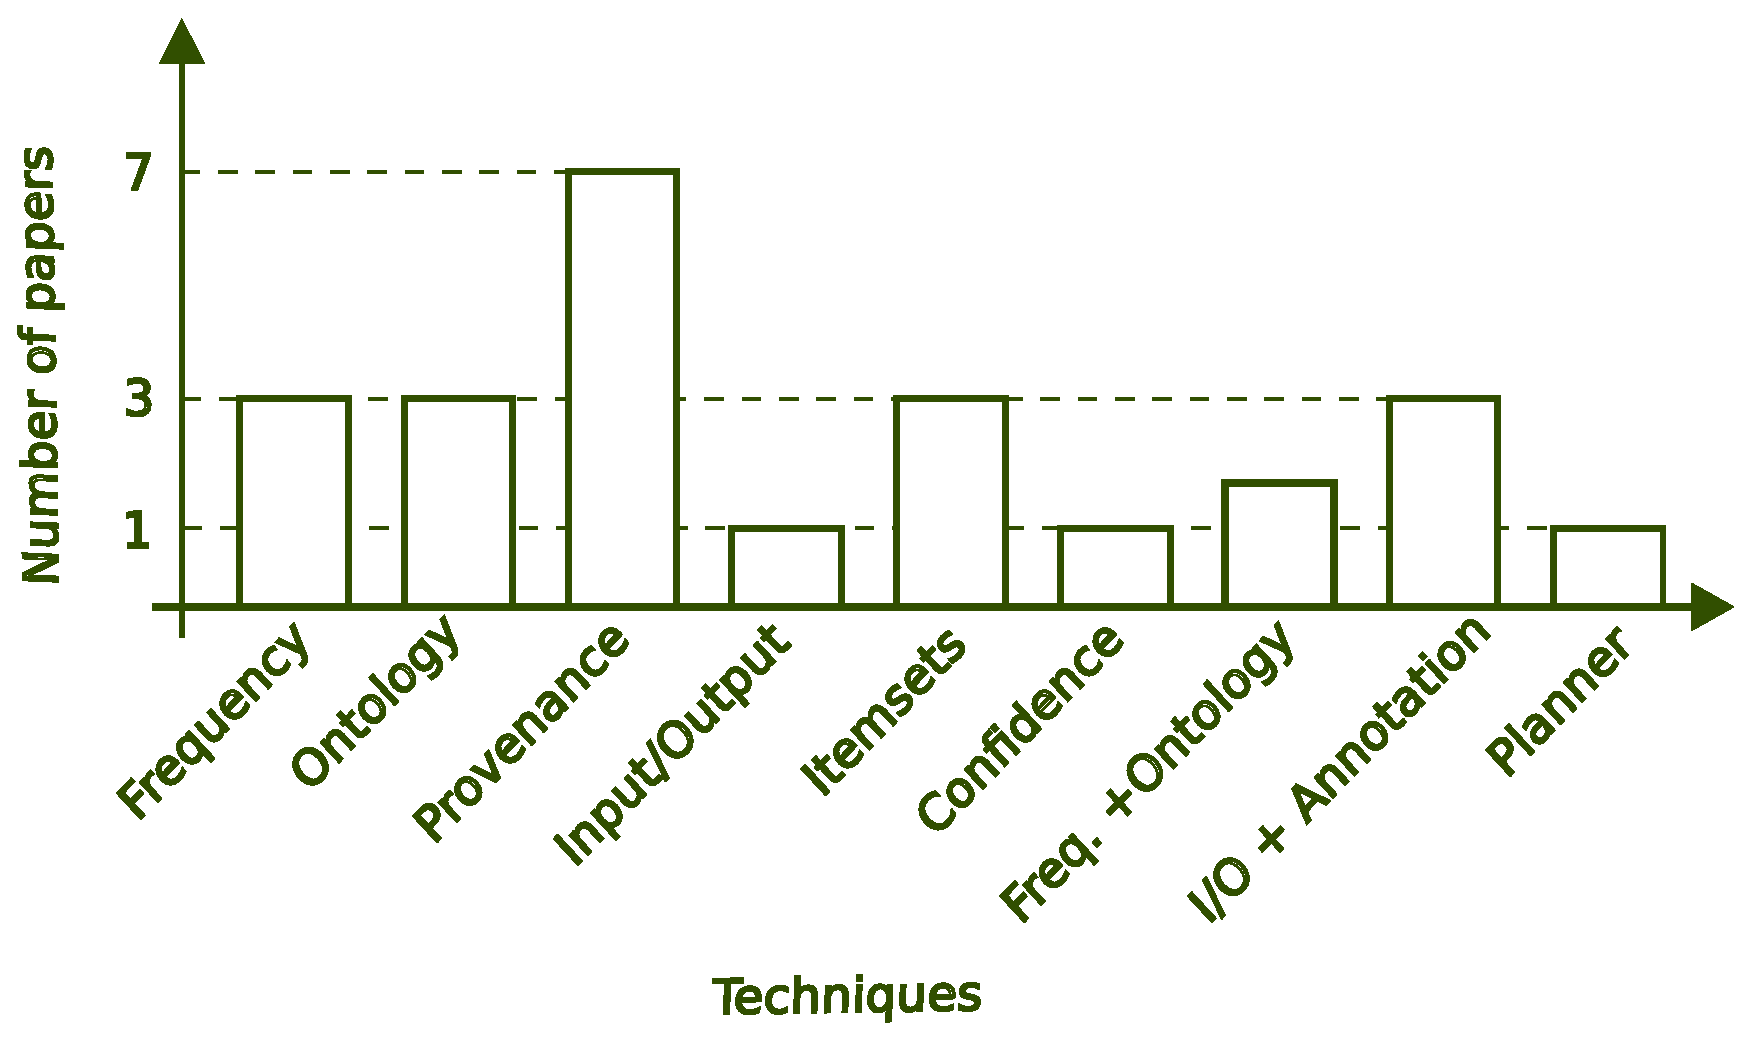
\includegraphics[height=15cm, width=28cm]{QuantidadeTecnicaVerdeForte.eps}
\end{center}

\section*{Main Contributions}

\subsection*{Recommendation as a classification problem}
We have downloaded $73$ bioinformatic's workflow's with their $280$ activities (from \emph{myExperiment}) were converted into a matrix $M_{i, j}$. In this matrix (we call it \emph{original dataset}), each line corresponds to a workflow and each column to an activity. $M_{i, j} = 1$ means that the workflows \emph{i} has the activity \emph{j}. Otherwise, $M_{i, j} = 0$ means that the workflow \emph{i} does not have the activity \emph{j}. To evaluate the approach, an activity is removed from each row of the original dataset, and a list of possible activities is recommended. The goal of the recommendation system is to correctly identify which activity is missing in the workflow (i.e., the one that was removed).

In order to use classification and regression techniques, some changes were proposed in the original dataset, which can be viewed in the next table. Each workflow was replicated \(118\) times. \(59\) of these correspond to identical copies of the original workflow, while in the other \(59\) one activity was removed from the original workflow and a new activity was added representing a possible recommendation. Thus, for each original workflow, there will be \(59\) correct instances and \(59\) incorrect instances and this type of information will be used to train the classifiers and the regressors. 
{ 
\color{darkgreen}
\vspace{0.25cm}
\begin{center}
\captionof*{table}{  \large \color{darkgreen} Adaptaded matrix for recommendation modeled \\ as classification/regression problem}
\vspace{0.25cm}
\begin{tabular}{|l|l|l|l|l|l|l|}  \hline
\textbf{\(\#\)} & \textbf{Workflow} & \textbf{Activ\(\mathbf{01}\)} &  
\textbf{\(\mathbf{\ldots}\)}  & \textbf{Activ\(\mathbf{280}\)} &\textbf{Class} 				\\ \hline

1    			& 01   	 		& 1 	   				& \(\ldots\)        & 0     			& T    				\\ \hline
2    			& 01      		& 1    				& \(\ldots\)        & 0     			& T  	  				\\ \hline
\(\vdots\)  	& \(\vdots\)    & \(\vdots\)    	& \(\vdots\)       & \(\vdots\)    & \(\vdots\)    	\\ \hline
59          	& 01     			& 1    				& \(\ldots\)        & 0     			& T             		\\ \hline
1    			& 01     			& 0 (removed)   & \(\ldots\)        & 0     			& F            		 	\\ \hline
2   			& 01     			& 0 (removed)   & \(\ldots\)        & 0     			& F            		 	\\ \hline
\(\vdots\)  	& \(\vdots\)    & \(\vdots\)    	& \(\vdots\)        & \(\vdots\)   & \(\vdots\)    	\\ \hline
59          	& 01     			& 0 (removed)   & \(\ldots\)        & 1 (added)   & F             		\\ \hline
1    			& 73     			& 1    				& \(\ldots\)        & 0     			& T             		\\ \hline
2    			& 73     			& 1    				& \(\ldots\)        & 0     			& T             		\\ \hline
\(\vdots\)  	& \(\vdots\)    & \(\vdots\)    	& \(\vdots\)        & \(\vdots\)   & \(\vdots\)    	\\ \hline
59          	& 73     			& 1    				& \(\ldots\)        & 0     			& T             		\\ \hline
1    			& 73     			& 1 (added)    	& \(\ldots\)        & 0     			& F           			\\ \hline
2    			& 73     			& 1   					& \(\ldots\)        & 0     			& F             		\\ \hline
\(\vdots\)  	& \(\vdots\)    & \(\vdots\)    	& \(\vdots\)        & \(\vdots\)   & \(\vdots\)    	\\ \hline
59          	& 73     			& 1    				& \(\ldots\)        & 1 (added)    & F             		\\ \hline

\end{tabular} \label{Tab_matriz_adaptada}
\end{center}
}
\vspace{0.25cm}

\subsection*{Recommendation Algorithm}
The proposed solution recommends activities using three concepts in the area of scientific workflows: i) frequency of activities; ii) compatibility between input and output; and iii) semantics of activities. The solution begins calculating the frequency of occurrence of each pair of existing activities, which is the number of times that an activity \emph{W} occurs immediately after another activity \emph{Z}. By considering only activities that have already been connected (on the dataset of workflows), the output and input compatibility is guaranteed.

After calculating the frequency it is necessary to annotate all the workflows, using the concepts of the domain ontology, this step was performed manually (not automatically). Finally, the algorithm annotates all activities with the same annotations of their respective workflow; i.e., if the \emph{X} activity is inside two workflows with distinct annotations, then this activity will be related to two different concepts from the ontology. 

To understand the recommendation training mechanism, another example will be used to simulate a user interacting with the recommendation system. Let us assume that during the construction of the workflow a scientist inserts the \emph{Z} activity and asks for a recommendation. The system will look at the list of activities after \emph{Z} sorted by frequency and ontological concept and will return the recommendation list. The sorting considers the ontological concepts serves as a tiebreaker criterion when two activities have the same frequency.
\vspace{0.25cm}
\begin{center}
\large  \color{darkgreen} Proposed solution \\
\vspace{0.25cm}
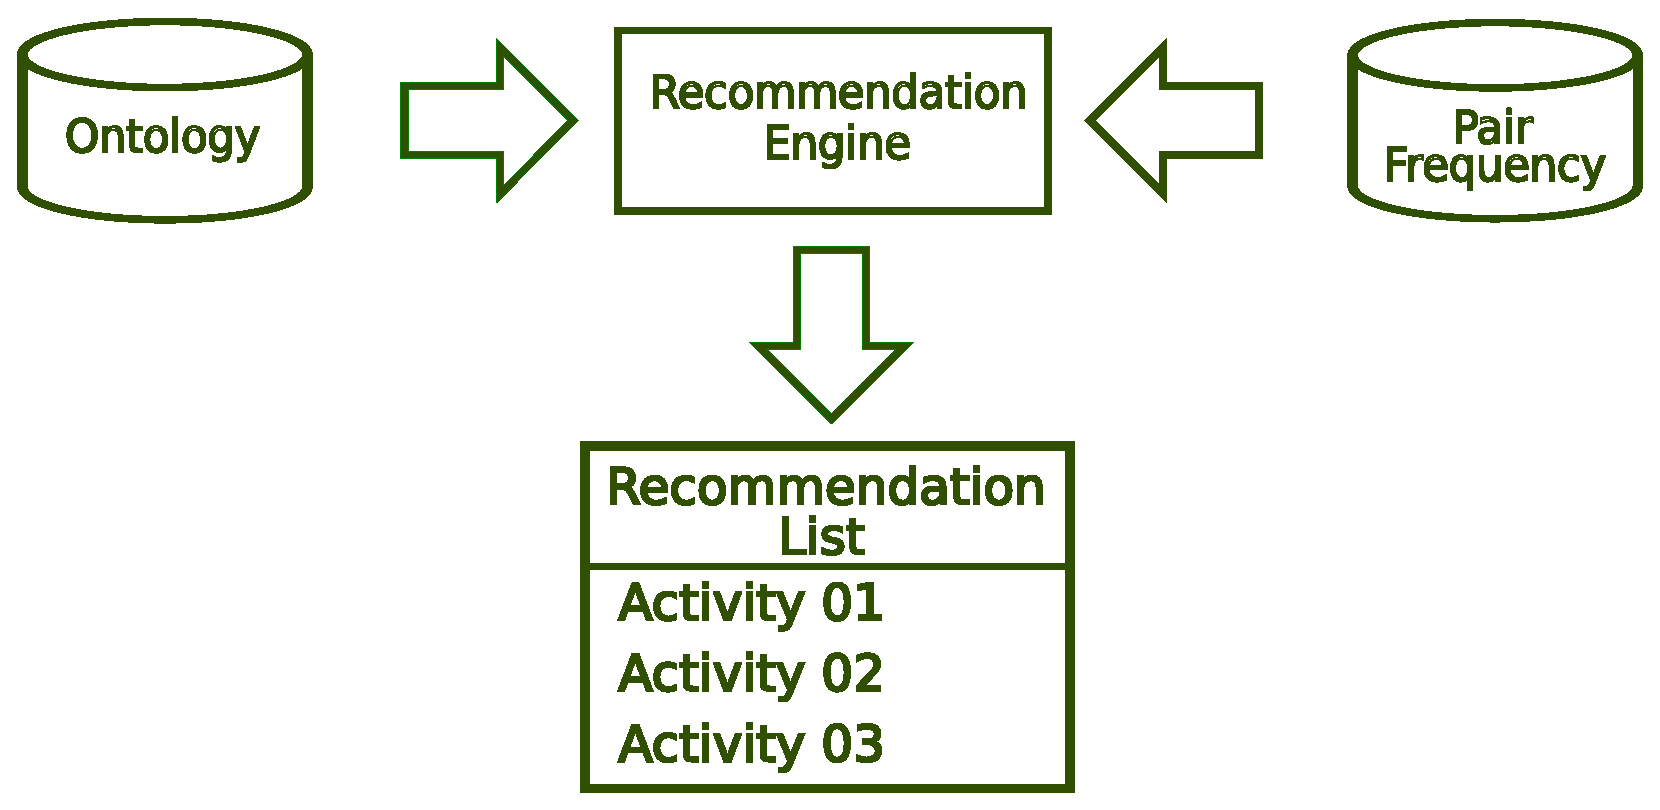
\includegraphics[height=15cm, width=28cm]{engineVerdeForte.eps}
\end{center}
\vspace{0.25cm}

%----------------------------------------------------------------------------------------
%	RESULTS 
%----------------------------------------------------------------------------------------

\section*{Results}
Our ontology-based approach (FESO) achieved better (or at least equal) results than the previous approaches for almost all of the evaluated metrics. It considers the use of frequency, input, output and semantic information about the activities, in comparison to the other techniques, its results were higher for all calculated metrics. Concerning the FES technique, its results were superior. In particular, part of this improvement is justified by cases where the correct activity has zero frequency in the training set. Since FESO considers the ontology information it is able to recommend activities even if they have zero frequency in the train set. In addition, for the cases where there is a tie between two activities considering the input, output, and the frequency criteria, the proposed technique presents an additional factor to be used as a tie breaker.

We were able to identify some trends in these results. Increasing information on data in the recommendation improves their recommendation performance, as the results of the experiments: $11$ and $16$ show. A second trend is that the SVM classifier was the only one that obtained a better result than the regressors. indicating that solutions by maximizing space between data in high dimension may be a promising area of study. A third trend is the use of composite classifiers and ensembles which presented promising results. 
{
\color{darkgreen}
\vspace{0.25cm}
\begin{center}
\captionof*{table}{ \large \color{darkgreen} Results of the recommendation modeled as \\ classification/regression problem}
\vspace{0.25cm}
\begin{tabular}{|l|l|l|l|l|l|} \hline
\textbf{\(\mathbf{\#}\)} & \textbf{Approach}&\textbf{S@1}&\textbf{S@5} & \textbf{S@10}  & \textbf{MRR} \\ \hline
		
1      & Random                             & 0.0037                        & 0.0260                        & 0.0280                         & 0.033          \\ \hline
2      & \emph{Apriori}    			& 0.0037                        & 0.0385                        & 0.0559                         & 0.037           \\ \hline
3      & KNN\(_C\)                         & 0.0037                        & 0.0685                        & 0.0959                         & 0.040           \\ \hline
4      & Neural Network\(_C\)      & 0.0137                         & 0.1507                        & 0.1781                           & 0.089           \\ \hline
5      & CART\(_C\)                       & 0.0274                        & 0.1233                        & 0.3699                          & 0.113            \\ \hline
6      & CART\(_R\)                       & 0.1370                         & 0.1370                        & 0.2603                          & 0.114            \\ \hline
7      & Naive Bayes\(_C\)            & 0.0274                        & 0.1507                        & 0.3425                          & 0.114            \\ \hline
8      & Binomial\(_R\)                  & 0.0822                        & 0.1918                         & 0.2055                          & 0.136            \\ \hline
9      & Neural Network\(_R\)      & 0.1096                        & 0.2603                        & 0.2603                          & 0.154            \\ \hline
10    & MARS\(_R\)                      & 0.1233                        & 0.2055                         & 0.2192                          & 0.167            \\ \hline
11     & FES                                  & 0.1474                        & 0.2603                         & 0.3699                          & 0.196           \\ \hline
12    & SVM\(_R\)                        & 0.1233                        & 0.3151                          & 0.4932                          & 0.238           \\ \hline
13    & SVM\(_C\)                        & 0.2425                        & 0.4658                        & 0.4932                          & 0.244           \\ \hline
14    & composed SVM\(_C\)     & 0.2515                        & 0.4458                         & 0.5232                          & 0.314            \\ \hline
15    & Rotation Forest\(_C\)      & 0.2925                        & 0.4558                        & 0.5432                          & 0.324            \\ \hline
16    & FESO                                & 0.3425                        & 0.4658                        & 0.5932                          & 0.334            \\ \hline

\end{tabular}
\end{center}
}
\vspace{0.25cm}

\section*{Conclusions}

This work developed a hybrid technique for recommending activities in scientific workflows which uses syntactic compatibility, frequency, and domain ontologies to recommend activities, called \emph{Frequency Input Output} (FESO, the number $16$ in the table above). Moreover, we have modeled the recommendation problem as a regression and classification problem in artificial intelligence. As future work we intend to investigate the use of data provenance to increase the accuracy of the recommendations.

\section*{Acknowledgements}

We thank the University of São Paulo and the CAPES, which provided scholarships for the student. 

%----------------------------------------------------------------------------------------

\end{multicols}
\end{document}